% Preamble
\documentclass[a4paper, 12pt]{article}
\usepackage[margin=1in]{geometry} % Set margin
\usepackage{pdfpages} % Insert pdf pages
\usepackage{amssymb,amsmath,amsthm, amsfonts} % Math libraries

% Custom commands
\newcommand{\sub}[1]{\subsection{\underline{#1}}}
\newcommand{\subsub}[1]{\subsubsection{\underline{#1}}}
\newcommand{\R}{\ensuremath{\mathbb{R}}}
\newcommand{\F}{\ensuremath{\mathbb{F}}}
\newcommand{\N}{\ensuremath{\mathbb{N}}}
\newcommand{\Onef}{\ensuremath{1_{\F}}}
\newcommand{\Zerof}{\ensuremath{0_{\F}}}
\newcommand{\eqbcuz}[1]{\text{~$\stackrel{(#1)}{=}$~}}
\newcommand{\eq}[1]{\begin{align*}#1\end{align*}}
\newcommand{\eqn}[1]{\begin{align}#1\end{align}}
\newcommand{\set}[1]{\big{\{} #1 \big{\}}}
\newcommand{\bigset}[1]{\bigg{\{} #1 \bigg{\}}}
\renewcommand{\qed}{\hfill\(\qedsymbol\)}
\newtheorem{lemma}{Lemma}

% Begin Document %
\begin{document}

% Title Page
\begin{titlepage}
    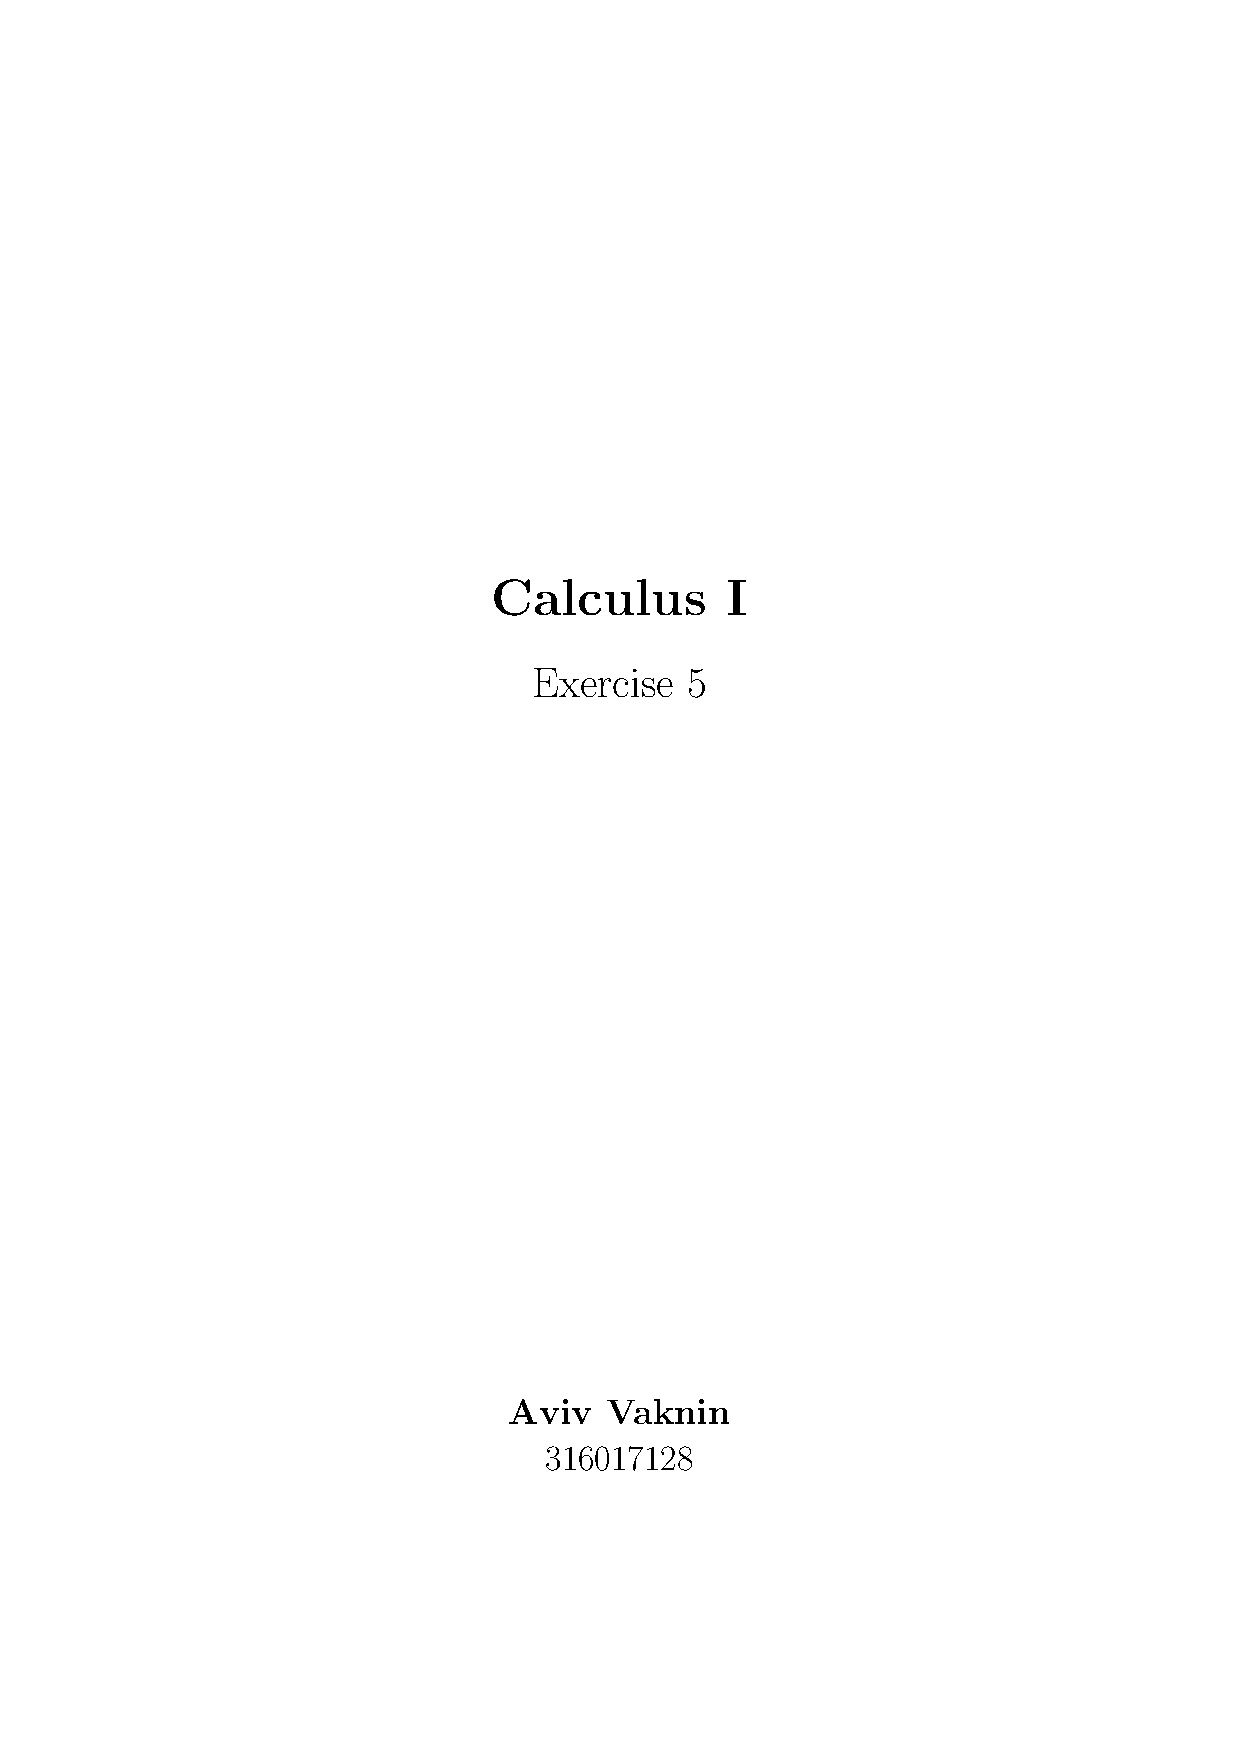
\includepdf{title.pdf}
\end{titlepage}

% 1
\section{Decide whether the following series converge or diverge.}
\setcounter{subsection}{1}
% 1.2
\sub{}
\eq{
    b_n=\frac
    {5+(-1)^nn}
    {4n^2+1}
}
$b_n$ converges to $0$.\\
Therefore, for every $\epsilon>0$ we need to find an $N\in\N$ such that for every $n>N$:
\eq{
    \bigg{|}
    \frac
    {5+(-1)^nn}
    {4n^2+1}
    -0
    \bigg{|}
    <\epsilon
}
Let $\epsilon>0$.\\
We'll choose $N\in\N$ such that:
\eq{
    N>\frac{2}{\epsilon}
}
For every natural $n>N$:
\eq{
    \frac{2}{n}<\frac{2}{N}
}
Therefore, for every $n>N$ we'll get:
\eq{
    \bigg{|}
    \frac
    {5+(-1)^nn}
    {4n^2+1}
    -0
    \bigg{|}
    <\frac{8n}{4n^2}
    =\frac{2}{n}
    <\frac{2}{N}
    <\frac{2}{\frac{2}{\epsilon}}
    =\epsilon
}
Thus, by definition:
\eq{
    lim(b_n)=0
}
\qed
% 1.3
\sub{}
\eq{
    c_n&=(n+1)^2-n^2\\
    &=n^2+2n+1-n^2\\
    &=2n+1\\
    &>n
}
$c_n$ is not bounded because $c_n>n$.\\
Because the series is not bounded, it diverges.
\qed\pagebreak
% 1.4
\sub{}
\eq{
    d_n=\frac
    {\sqrt{16n^2+3}}
    {n}
}
Let $\epsilon>0$.\\
We'll choose $N\in\N$ such that:
\eq{
    N>\frac{1}{\epsilon}
}
And that for every natural $n>N$:
\eq{
    \frac{1}{n}<\frac{1}{N}
}
Therefore, for every $n>N$ we'll get:
\eq{
    \bigg{|}
    \frac
    {\sqrt{16n^2+3}}
    {n}
    -4
    \bigg{|}
    <\frac{1}{n}
    <\frac{1}{N}
    <\frac{1}{\frac{1}{\epsilon}}
    =\epsilon
}
Thus, by definition:
\eq{
    lim(d_n)=4
}
\qed

% 2
\section{}
\sub{Write formally: $(an)_{n=1}^\infty$ converges}
\eq{
    \exists{L}\in\R~~~\forall\epsilon>0~~~\exists{N}\in\N~~~\forall{n}>N~~~|a_n-L|<\epsilon
}
\sub{Write formally: $(an)_{n=1}^\infty$ not converges}
\eq{
    \forall{L}\in\R~~~\exists\epsilon>0~~~\forall{N}\in\N~~~\exists{n}>N~~~|a_n-L|\geq\epsilon
}
\sub{Prove $a_n$ diverges}
\eq{
    a_n=\bigg{\{}
    \begin{matrix}
        1+\frac{1}{n}&n~is~even\\
        2&n~is~odd
    \end{matrix}
}
Although $a_n$ is bounded, it diverges.\\
We can see that because for even \textit{n}'s, the values will keep getting smaller and smaller, but never smaller than 1.\\
Therefore, $\lim(1+\frac{1}{n})=1$.\\
In addition, while n is odd, we'll get the permanent series $2$, whose limit is $lim(2)=2$.\\
However, as we're constantly "moving" between two different limits, we can see that the definition of the limit won't hold for any of the limits, i.e. 1 \textit{or} 2.\\
Therefore, neither of them is the limit of the series, and the series diverges.
\qed\pagebreak

% 3
\section{Prove or disprove}
\setcounter{subsection}{1}
\sub{}
The statement is incorrect.\\
As an example, let $a_n$ be:
\eq{
    a_n=1^n
}
Therefore, $a_n$ diverges as it doesn't converge into a single value.\\
In other words, for any $\epsilon>0$ there doesn't exist $N\in\N$ such that $\forall{n}>N~~|a_n-L|<\epsilon$.
On the other hand, $|a_n|$ converges to $1$, and therefore:
\eq{
    lim(|a_n|)=1
}
\qed
\setcounter{subsection}{3}
\sub{}
The statement is correct.\\
The regular definition of the limit is: "$\forall\epsilon>0~~~\exists{N}\in\N$",
which states that for any possible $\epsilon$ - as small or as big as we might find,
we'll always be able to find some $N$.\\
However, this statement is \textbf{more strict}.\\
According to the statement, an $N\in\N$ exists that satisfies the definition for \textbf{every} $\epsilon$.\\
Therefore, it doesn't contradict the traditional definition of the limit, and we can assume that:
\eq{
    lim(a_n)=L
}
\qed
\pagebreak

% 4
\section{$a_n$ converges to $L\in\R$, prove the following:}
\sub{$L\geq{0}$}
Let's assume by contradiction that $L<0$.\\
Let $\lambda\in\R$ such that:
\eq{
    &\lambda=\frac{L}{2}\\
    &L<\lambda<0
}
According to (10.9) from lecture, we can assume that from a certain point, $a_n<\lambda$.\\
However, we've reached a contradiction:
\eq{
    &0\leq a_n<\lambda<0
}
Therefore, we've proved that $L\geq{0}$.
\qed
\sub{$L=0\implies lim(\sqrt{a_n})=0$}
It is given that $(a_n)$ converges to 0 as $L=0$.\\
Therefore by definition, for any arbitrary $\epsilon>0$, we'll be able to find some $N\in\N$ such that $\forall{n}>N$:
\eq{
    |a_n|<\epsilon
}
$(\sqrt{a_n})$ is the same series, but every member in the series is being rooted.\\
Therefore, for \textbf{that same} $N$, every $n>N$ will converge as well, to $\sqrt{0}=0$:
\eq{
    lim(\sqrt{a_n})=\sqrt{0}=0
}
\qed
\sub{$L>0\implies lim(\sqrt{a_n})=\sqrt{L}$}
Similarly to 4.2, we know that $(\sqrt{a_n})$ is the same series, but every member in the series is being rooted.\\
Therefore, for \textbf{that same} $N$, every $n>N$ will converge as well.\\
This time however, we know that $L>0$, and therefore $(a_n)$ converges to a number that is bigger than 0, which is $L$.\\
Therefore, $(\sqrt{a_n})$ converges to the square root of a number that is bigger than 0 - which is L, that is:
\eq{
    lim(\sqrt{a_n})=\sqrt{lim(a_n)}=\sqrt{L}
}
\qed\pagebreak

% 5
\section{}
\setcounter{subsection}{1}
\sub{}
We learn from 5.1, that once we take any sequence of the form $a_n=x^n$, as long as $x>0$, at "very large" numbers, $a_n$ will be "very large".\\
Thus, $a_n$ diverges, as it keeps increasing - exponentially.\\
Therefore, once we try to calculate the limit of $\frac{1}{x^n}$:
\eq{
    a_n&=\frac{1}{x^n}\\
    lim(a_n)&=0
}
In addition, using the fact that $x^n$ is exponentially bigger than $n$, and the law of limits division:
\eq{
    lim(n)&=n\\
    lim(\frac{n}{x^n})&=0\\
}
\sub{}
We need to prove the following:
\eq{
    \sqrt[n]{n}<1+\sqrt{\frac{2}{n-1}}
}
Let:
\eq{
    x=\sqrt{\frac{2}{n-1}}>0
}
According to (5.1):
\eq{
    (1+x)^n&>\frac{n(n-1)}{2}\cdot{x^2}\\
    &=\frac{n(n-1)}{2}\cdot\frac{2}{n-1}\\
    &=n
}
Notice that we were able to divide by $(n-1)$ as it is given that $2\leq{n}\in\N$.\\
We'll take the \textbf{n-th root} of both sides of the equation,\\
By utilizing what we've proved in exercise 2 question 8: $a>b\implies a^n>b^n$
\eq{
    (1+x)^n&>n\\
    1+x&>\sqrt[n]{n}\\
    1+\sqrt{\frac{2}{n-1}}&>\sqrt[n]{n}
}
\qed\pagebreak
\sub{}
We need to prove:
\eq{
    \lim(\sqrt[n]{n})=1
}
Therefore, we need to show that $\forall\epsilon>0~~\exists{N}\in\N~~\forall{n}>N$:
\eq{
    \bigg|\sqrt[n]{n}-1\bigg|<\epsilon
}
in (5.3) we've shown that:
\eqn{
    \sqrt[n]{n}<1+\sqrt{\frac{2}{n-1}}
}
Using (1) we can see:
\eqn{
    \sqrt[n]{n}-1<\sqrt{\frac{2}{n-1}}
}
Now, we can use (2) to bound the term from above:
\eq{
    \bigg|\sqrt[n]{n}-1\bigg|&=\sqrt[n]{n}-1\\
    &<\sqrt{\frac{2}{n-1}}\\
    &<\frac{2}{n-1}
}
Therefore, for every $N>\frac{2}{\epsilon}+1$:
\eq{
    \bigg|\sqrt[n]{n}-1\bigg|&<\frac{2}{n-1}\\
    &<\frac{2}{N-1}\\
    &<\frac{2}{\frac{2}{\epsilon}+1-1}\\
    &=\epsilon
}
Therefore, by the limit's definition:
\eq{
    \lim(\sqrt[n]{n})=1
}
\qed\pagebreak

% 6
\section{}
\sub{}
The statement is \textbf{true}.\\
It is given that ($a_n$) and ($a_n+b_n$) converge, therefore, both of them have limits.\\
By definition, the limit of the sum of sequences, is the sum of the limits, therefore:
\eq{
    &\lim(a_n+b_n)=\lim(a_n)+\lim(b_n)\\
    &\lim(b_n)=\lim(a_n+b_n)-\lim(a_n)
}
Therefore, we can conclude that $b_n$ converges.
\qed
\sub{}
The statement is \textbf{false}, here's an example:
\eq{
    &a_n=\frac{1}{n^2}\\
    &b_n=n\\
    &a_n\cdot b_n=\frac{n}{n^2}=\frac{1}{n}
}
We can clearly see that $a_n$ and $a_n\cdot b_n$ converge to 0, yet $b_n$ diverges.
\qed
\sub{}
The statement is \textbf{false}.\\
As an example, let's define $a_n$ and $b_n$:
\eq{
    a_n=\bigg{\{}\begin{matrix}
        n & \text{n is odd}\\
        \frac{1}{n^2} & \text{n is even}\\
    \end{matrix}
    \\
    b_n=\bigg{\{}\begin{matrix}
        \frac{1}{n^2} & \text{n is odd}\\
        n & \text{n is even}\\
    \end{matrix}
}
Now, we can clearly see that both of these sequences do not converge and therefore - do not have limits.\\
However, we can see that $a_nb_n$ \textbf{does} converge, and it converges to $0$.
\qed
% \sub{6.3 old}
% We'll prove this using contraposition.\\
% Let:
% \eq{
%     c_n=a_nb_n
% }
% We'll assume $\lim(a_n)\neq{0}$ \textbf{and} $\lim(b_n)\neq{0}$ and show that the limit of $c_n$ cannot equal $0$.\\
% According to the limit multiplication rule:
% \eq{
%     \lim(c_n)=\lim(a_n)\cdot\lim(b_n)\neq{0}
% }
% Due to the uniqueness of zero, the only way that $c_n$ can equal zero, is if at least one of the multiplication factors is zero.\\
% However, because we assumed that both of the factors are not zero, $\lim(c_n)$ cannot equal zero.\\
% Thus, we've shown that if \textbf{both} of the limits are not zero, their multiplication cannot be zero, that is:
% \eq{
%     \lim(a_n)\neq{0}~~\land~~\lim(b_n)\neq{0}\implies\lim(c_n)\neq{0}
% }
% Which is the contrapositive form of what we were trying to prove.
% \qed
\pagebreak

% 7
\section{}
\sub{}
Let:
\eq{
    G&=\sqrt[n]{y_1\cdot...\cdot y_n}\\
    S&=y_1+...+y_n
}
We need to prove:
\eq{
    G\leq\frac{S}{n}
}
First, we'll show:
\eq{
    \prod^{n}_{i=1}\frac{y_i}{G}=1
}
\eq{
    \prod^{n}_{i=1}\frac{y_i}{G}&=\frac{y_1\cdot...\cdot y_n}{G^n}\\
    &=\frac{y_1\cdot...\cdot y_n}{(\sqrt[n]{y_1\cdot...\cdot y_n})^n}\\
    &=\frac{y_1\cdot...\cdot y_n}{y_1\cdot...\cdot y_n}\\
    &=1\\
}
This will let us use the assumption from question 7 on exercise 4:
\eq{
    \prod^{n}_{i=1}\frac{y_i}{G}=1 \implies \sum^{n}_{i=1}\frac{y_i}{G}\geq{n}
}
Therefore:
\eq{
    \sum^{n}_{i=1}\frac{y_i}{G}&=\frac{y_1+...+y_n}{G}\\
    &=\frac{S}{G}\geq{n}
}
Now we can apply some inequality algebra:
\eq{
    \frac{G}{S}&\leq\frac{1}{n}\\
    G&\leq\frac{S}{n}\\
}
\qed

% End
\end{document}